\chapter{Anvendelsesgrænsetilstand}
Nu er brudgrænsetilstanden bestemt, i det følgende regnes anvendelsesgrænsetilstanden. Ud fra anvendelsesgrænsetilstanden kan det vurderes, om bygningen har tilstrækkelig små deformationer til, at bygningens dimensioner kan godtages. 
\newline \indent{     }  Det antages, at der kun virker én variabel last på konstruktionen, nemlig vindlasten. Denne last forlænges helt ned til understøtningerne, og der ses bort fra jordlasten. Derfor er der udregnet nye reaktioner for konstruktionen, som ses i Tabel \ref{tab:anden}. Beregningerne kan ses i Bilag XX. 

\begin{table}
	\begin{center}
		\begin{tabular}{|c|c|c|}
			\hline
			Reaktion & Værdi & Enhed \\ \hline
			$S_x$ & -71,14 		& kN      \\ \hline
			$C_y$ & 578,86 		& kN      \\ \hline
			$S_y$ & 36,07 		& kN       \\ \hline
			$B_y$ & 1432,31 	& kN      \\ \hline
			$A_y$ & 344,53 		& kN      \\ \hline
			$B_x$ & 0,00 		& kN      \\ \hline
			$A_x$ & -147,87 	& kN       \\ \hline
		\end{tabular}
		\caption{Reaktioner for anvendelsesgrænsetilstand}
		\label{tab:anden}
	\end{center}
\end{table}

\section{Snitkræfter}
Der er lavet i alt fem snit på konstruktionen, som vist på Figur \ref{fig:snitanvendelse}. Dog ses der bort fra den højre del af konstruktionen, og dermed er det kun snit 1-3 der anvendes. 

\begin{figure}[H]
	\centering
	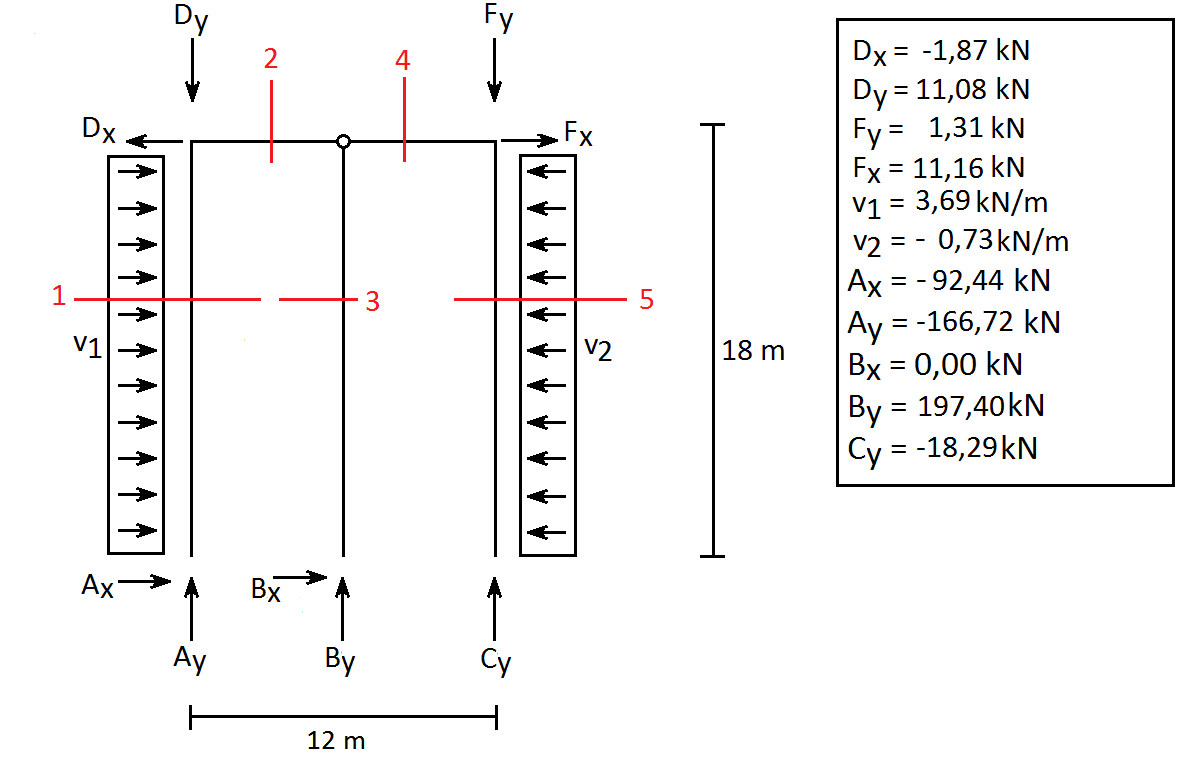
\includegraphics[width=0.9\textwidth]{billeder/snitanvendelse.png}
	\caption{Snit}
	\label{fig:snitanvendelse}
\end{figure}

Nedenfor er vist et eksempel på, hvordan snitkræfterne regnes for snit 1. Alle beregningerne findes i Bilag XX og resultaterne for alle snitkræfter kan ses i Tabel \ref{tab:anden2}.
\newline
\newline
\textbf{Snit 1: 0 m < x < 18 m}
\newline
Fritlegemediagrammet for snit 1 ses på Figur \ref{fig:snitetan}.
\begin{figure}[H]
	\centering
	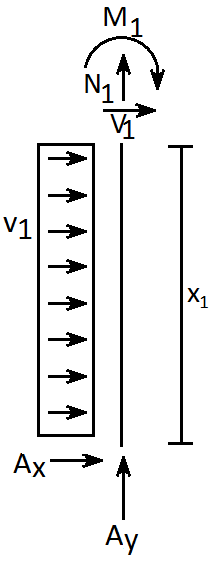
\includegraphics[width=0.2\textwidth]{billeder/asnitet.png}
	\caption{Snit 1}
	\label{fig:snitetan}
\end{figure}

Først bestemmes normalkraften:
\begin{center}
	$0 = N_1 + A_y - E_1\cdot x \leftrightarrow N_1(x) = 31,\cdot54 \frac{kN}{m} \cdot x - 886,\!36 kN$
\end{center}

Normalkraften bestemmes ved 0 m og 18 m:
\begin{center}
	$N_1(0m) = -886,\!36 kN$ og $N_1(18m) = -318,\!62 kN$
\end{center}

Nu bestemmes forskydningskraften:
\begin{center}
	$0 = V_1 + A_x + Vind_1 \cdot x \leftrightarrow V_1(x) = -6,\!08 \frac{kN}{m} \cdot x + 147,\!87$
\end{center}

Forskydningskraften bestemmes ved 0 m og 18 m:
\begin{center}
	$V_1(0m) = 147,\!87$ og $V_1(18m) = 38,\!39$
\end{center}

Til sidst bestemmes momentkraften:
\begin{center}
	$0 = M_1 + A_x \cdot x + Vind_1\cdot x\cdot \frac{x}{2} \leftrightarrow M_1(x) = 147,\!87 kN\cdot x - 3,\!04 \frac{kN}{m}\cdot x^2$
\end{center}

Momentkraften bestemmes ved 0 m og 18 m:
\begin{center}
	$M_1(0m) = 0,\!00 kNm$ og $M_1(18m) = 1676,\!36 kNm$
\end{center}

\begin{table}
	\begin{center}
		\begin{tabular}{|c|c|c|c|c|c|c|}
			\hline
			Snit/Værdi & N($x_{min}$) & N($x_{max}$) & V($x_{min}$) & V($x_{max}$) & M($x_{min}$) & M($x_{max}$) 	\\ \hline
			1. A-D, 0<x<18 	& -886,36 	& -318,62 	&  147,87 	&  38,39 	&  0,00     &  1676,36        		\\ \hline
			2. D-E, 0<x<6  	&  71,14    &  71,14    &  275,67   & -283,12   &  1676,36  &  0,00    \\ \hline
			3. B-E, 0<x<18  & -948,58   &  164,54   &  0,00     &  0,00     &  0,00     &  0,00 			    \\ \hline
			4. E-F, 0<x<6   &  71,00    &  71,00    &  28,62    &  36,07    &  194,06   &  0,00     \\ \hline
			5. C-F, 0<x<18     & -578,86   & -11,12    &  0,00     &  21,56    &  0,00     &  194,06       		\\ \hline
		\end{tabular}
		\caption{Snitkræfter for anvendelsesgrænsetilstand, N og V: kN og M: $kNm$}
		\label{tab:anden2}
	\end{center}
\end{table}

\section{Bjælkens differentialligning}
For at udregne udbøjningerne for stængerne, anvendes bjælkens differentialligning. Da det statiske system for tilbygningen til Strøybergs Palæ er statisk bestemt, er det den anden ordens afledede, som anvendes for at bestemme udbøjningerne.